\chapter{Finding Data}
\label{ch:finding}

\section{Find}
\index{find}

Press \keyc{Ctrl}{F}, or choose \menupath{Edit > Find}.

A prompt appears on the bottom line of the screen, with an underscore marking
where the next character will go:

\begin{ccfigure}
\ccscreenscale{1.5}
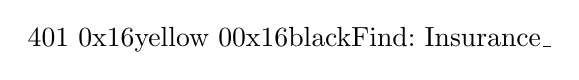
\begin{tikzpicture}
\node[inner sep=0pt,anchor=north west] (fd) at (0,0) {%
\ccscreenbegin{40}{1}
  \ccfillrow{0}{x16yellow}
  \cctext{0}{0}{x16black}{Find:~Insurance\_}
\ccscreenend
};
\end{tikzpicture}
\caption{The Find prompt}
\label{fig:find}
\end{ccfigure}

Type what you are looking for and press \key{Return}. \ccprod{} moves the
cursor to the next cell containing it.

\begin{cctable}{Key}{Effect}{1.55in}{3.27in}
Any printable key & Adds a character to the search text \\
\key{Backspace} & Removes the last character \\
\key{Return} & Searches, if there is anything to search for \\
\key{Esc} & Abandons the search \\
\end{cctable}

The prompt takes at most \textbf{fifteen} characters. It has no insertion point
and no arrow keys: you type forwards and delete backwards, and that is all.

\section{What Find matches}

\begin{ccsteps}
\item \textbf{Anywhere in the cell.} Searching for \lit{sur} finds
\lit{Insurance}. It is a substring search, not a whole-cell match.
\item \textbf{Ignoring case.} \lit{insurance}, \lit{Insurance} and
\lit{INSURANCE} all find each other.
\item \textbf{What the cell displays}, not what it contains. A cell holding
\fml{=SUM(B2:B7)} and showing \lit{13388.2} is found by searching for
\lit{13388}. Searching for \lit{SUM} will not find it.
\item \textbf{The current worksheet only.} The other fifteen are not searched.
\item \textbf{The first 31 characters} of the cell's displayed text. Anything
past that is not looked at.
\end{ccsteps}

\section{Finding the next one}
\index{find!repeating}

There is no separate \menupath{Find Next} command, and there does not need to be
one. \ccprod{} looks for the first match that comes \emph{after} the cursor ---
reading the worksheet row by row, and left to right within a row --- and if
there is no such match it goes back to the first one anywhere on the worksheet.

Two things follow.

\begin{ccsteps}
\item \textbf{Repeating the command walks the matches.} Each search starts from
wherever the last one left the cursor, so the cursor steps through every match
in turn and then wraps round to the first.
\item \textbf{The search text is remembered.} The next time you press
\keyc{Ctrl}{F} the prompt already contains what you typed last time, so
\keyc{Ctrl}{F} followed by \key{Return} is the whole of ``find the next one''.
\end{ccsteps}

\begin{cccaution}
\textbf{A search that finds nothing says nothing.} The prompt disappears and the
cursor stays exactly where it was. There is no \msg{not found} message and no
sound.

That makes ``no match anywhere'' and ``the only match is the cell I am already
on'' look identical --- in both cases the cursor does not move. If you are not
sure which has happened, move the cursor off the cell and search again.
\end{cccaution}

\section{Replace}
\index{replace}\index{find!and replace}

Choose \menupath{Edit > Replace\ccdots}. There is no keyboard shortcut.

\ccprod{} asks two questions on the bottom line, one after the other:

\begin{ccfigure}
\ccscreenscale{1.5}
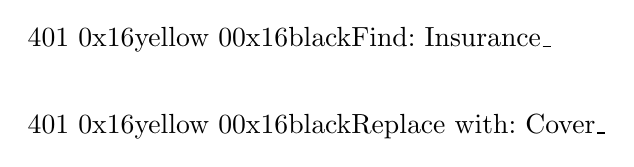
\begin{tikzpicture}
\node[inner sep=0pt,anchor=north west] (r1) at (0,0) {%
\ccscreenbegin{40}{1}
  \ccfillrow{0}{x16yellow}
  \cctext{0}{0}{x16black}{Find:~Insurance\_}
\ccscreenend
};
\node[inner sep=0pt,anchor=north west] (r2) at (0,-1.1) {%
\ccscreenbegin{40}{1}
  \ccfillrow{0}{x16yellow}
  \cctext{0}{0}{x16black}{Replace~with:~Cover\_}
\ccscreenend
};
\end{tikzpicture}
\caption{The two Replace prompts}
\label{fig:replace}
\end{ccfigure}

Both take at most fifteen characters and behave exactly like the \menupath{Find}
prompt --- type forwards, \key{Backspace} to delete, \key{Return} to accept,
\key{Esc} to abandon the whole command.

\textbf{The replacement may be empty.} Press \key{Return} at the second prompt
without typing anything and every match is deleted rather than replaced.

\subsection{Answering for each cell}

\ccprod{} does not change anything without asking. It searches the worksheet,
and for each cell it finds it moves the cursor there --- so you can see what is
about to change --- and asks:

\begin{ccfigure}
\ccscreenscale{1.5}
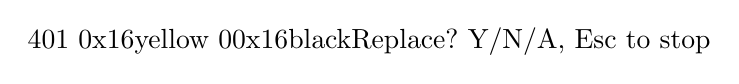
\begin{tikzpicture}
\node[inner sep=0pt,anchor=north west] (rq) at (0,0) {%
\ccscreenbegin{40}{1}
  \ccfillrow{0}{x16yellow}
  \cctext{0}{0}{x16black}{Replace?~Y/N/A,~Esc~to~stop}
\ccscreenend
};
\end{tikzpicture}
\caption{The question asked at each match}
\label{fig:replaceask}
\end{ccfigure}

\begin{cctable}{Key}{Effect}{1.55in}{3.27in}
\key{Y} & Replace this one, then go on to the next \\
\key{N}, or any other key & Leave this one alone, then go on to the next \\
\key{A} & Replace this one and \textbf{every remaining match}, without asking
again \\
\key{Esc} & Stop here. Everything already replaced stays replaced \\
\end{cctable}

\begin{cccaution}
\textbf{There is no undo.} \key{F5} does not reach a replacement, and neither
does anything else. That is why the command asks cell by cell, and it is worth
answering \key{Y} a few times before reaching for \key{A}.

Save the workbook before a large replacement. If it goes wrong, the way back is
to open the saved copy.
\end{cccaution}

\section{What Replace matches}

Mostly the same rules as \menupath{Find}, with three differences that matter.

\begin{ccsteps}
\item \textbf{The whole worksheet, from \cellref{A1}.} Unlike \menupath{Find},
which starts at the cursor, \menupath{Replace} always sweeps the used range from
the beginning --- left to right along each row, then down. Where the cursor
happens to be makes no difference.
\item \textbf{Formula cells are never touched.} A formula is skipped whether or
not its text matches. Searching for \lit{B2} will not rewrite \fml{=SUM(B2:B7)},
and a careless replacement cannot destroy your formulas.
\item \textbf{Every occurrence within a cell} is replaced, not just the first.
Replacing \lit{o} with \lit{0} turns \lit{London Office} into
\lit{L0nd0n 0ffice}.
\item \textbf{Ignoring case}, like \menupath{Find} --- but the replacement is
inserted exactly as you typed it. Replacing \lit{jan} with \lit{Jan} tidies
\lit{JAN} and \lit{jan} alike.
\item \textbf{Numbers as well as text.} What is matched is the cell's contents
as the formula bar shows them, so searching a sheet of figures for \lit{222}
finds them.
\end{ccsteps}

\begin{ccnote}
A replacement can change what kind of cell it is, exactly as retyping would.
Replacing \lit{222} with \lit{999} leaves a number; replacing it with
\lit{9x9} leaves text, because \lit{9x9} is not a number. The cell is re-read
from scratch, not patched.
\end{ccnote}

\begin{ccnote}
A cell whose contents run past 63 characters is skipped rather than truncated,
and so is any replacement that would push a cell past that length. Nothing is
said when this happens --- the cell is simply left alone.
\end{ccnote}

\section{Finding your way around instead}

For the common case --- getting back to a part of a large worksheet --- the
navigation keys are usually quicker than Find:

\begin{cctable}{To get to}{Press}{2.2in}{2.62in}
The top left of the worksheet & \keyc{Shift}{Home} \\
The start of the current row & \key{Home} \\
A screen at a time & \key{PgUp} and \key{PgDn} \\
A particular cell you can see & Click on it \\
\end{cctable}

There is no \menupath{Go to} command: you cannot type \cellref{B400} and be
taken there.
